\documentclass{deliverablereport}

\usepackage[style=alphabetic,backend=bibtex]{biblatex}
\usepackage{wrapfig}
\addbibresource{../../lib/kbibs/kwarcpubs.bib}
\addbibresource{../../lib/kbibs/extpubs.bib}
\addbibresource{../../lib/kbibs/kwarccrossrefs.bib}
\addbibresource{../../lib/kbibs/extcrossrefs.bib}
\addbibresource{../../lib/deliverables.bib}
%\addbibresource{../../lib/publications.bib}
\addbibresource{rest.bib}
% temporary fix due to http://tex.stackexchange.com/questions/311426/bibliography-error-use-of-blxbblverbaddi-doesnt-match-its-definition-ve
\makeatletter\def\blx@maxline{77}\makeatother

\deliverable{UI}{jupyter-test}
\deliverydate{02/27/2017}
\duedate{02/27/2017 (Month 18)}
\def\pn{OpenDreamKit}
\author{Martin Sandve Aln\ae{}s \& Hans Fangohr \& Vidar Fauske \& Thomas Kluyver \& Benjamin Ragan-Kelley \& MORE?}

\begin{document}
\maketitle
%  Work Package WP6 develops a novel, foundational, knowledge-based framework for
  interfacing existing open source mathematical software systems and knowledge bases into
  a mathematical VRE, where systems can delegate functionalities among each other
  seamlessly without losing semantics.

  The overall Math-in-the-Middle (MitM) Framework developed in WP6 over the last three
  years is described in D6.5; this Report complements it by describing the curated
  contents Math-in-the-Middle (MitM) Ontology which serves as a reference and pivotal
  point for translations between the various input languages of mathematical software
  systems and knowledge bases.

  In a nutshell, the MitM Ontology describes the mathematical objects, concepts, and their
  relations in a general, system-agnostic way in an OMDoc/MMT theory graph while the
  mathematical systems export API theories that describe the system interface language in
  terms of types, classes, constructors, and functions -- again in OMDoc/MMT. These two
  levels of descriptions are linked by OMDoc/MMT alignments that allow the translation of
  expressions between systems.

%%% Local Variables:
%%% mode: visual-line
%%% fill-column: 5000
%%% mode: latex 
%%% TeX-master: "report"
%%% End:

\strut\githubissuedescription
\newpage\tableofcontents\newpage

\newcommand{\nbval}{\texttt{nbval} }

\section{Background} % (fold)

\subsection{Jupyter notebook}
The Jupyter Notebook is a web application that enables the creation
and sharing of executable documents that contain live code,
equations, visualizations and explanatory text.


% \begin{wrapfigure}{r}{1.0\textwidth}
\begin{figure}
\centerline{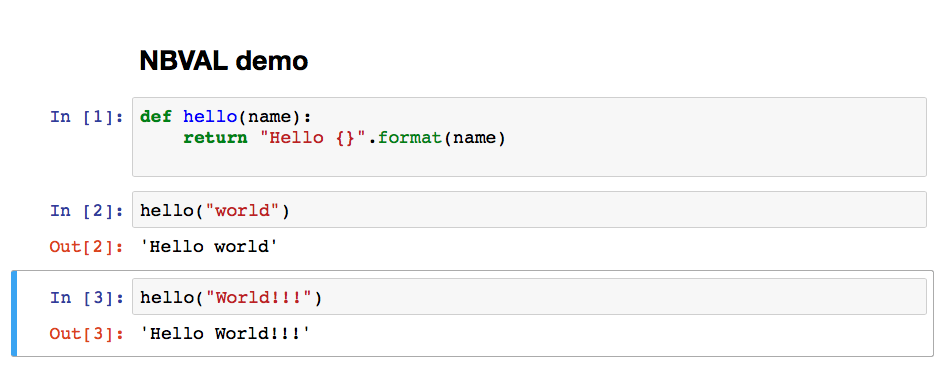
\includegraphics[width=1.0\textwidth]{examples/demo.png}}
\caption{\label{fig:jupyterdemo} Self-contained \Jupyter Notebook
  demonstrating the concepts of cells that contain different types of
  material and can be executed (or updated) in arbitrary or sequential
  order.}
\end{figure}
%\end{wrapfigure}

Thanks to a modular design, Jupyter notebooks can be used with any
computational system that provides a so-called Jupyter kernel
implementing the Jupyter messaging protocol to communicate with the
notebook. OpenDreamKit therefore promotes the Jupyter notebook as user
interface of choice, in particular since it is particularly suitable
for building modular web based Virtual Research Environments.

An example Jupyter notebook (using a Python kernel) is shown in
figure~\ref{fig:jupyterdemo}. Once the calculation, exploration and
annotation is completed, the document can be saved to disk as a (json)
file. This notebook can be opened again later at the same or different
computers, and will display input and output data as visible in the
figure. Furthermore, if a Python kernel is installed, the notebook can
be executed again  - thus providing an executable document, that
can integrate text, equations, code, output from the code, and graphs and
other multimedia objects.

The very nature of the notebook enables and encourages reproducible
science, contributing to our overall ambition of enabling better
science through better electronic infrastructure: researchers can
carry out a computation within the notebook, and all steps are
automatically recorded and can be saved at the press of a
button. While some editing (and maybe removing avenues of
computational exploration that were unsuccessful from the notebook) is
necessary before the notebook can be shared with others effectively,
this is still a significant advancement over managing snippets of
code, post processing scripts, figures and (latex) manuscripts in
different files and with no explicitly documented dependency.

We see Jupyter notebooks being used in a number of use cases, including
\begin{itemize}
\item computational exploration
\item documentation of software packages
\item tutorials for software
\item teaching materials in higher education
\end{itemize}

In this deliverable, we enrich the ecosystem of Jupyter notebook tools
with the NoteBook VALidation tool (\nbval), that allows to check the
types of documents listed above \emph{automatically} for they validity.

\subsection{Testing} % (fold)
\label{sec:testing}


It is good practice to test computer code through so-called unit
tests: for every functionality a code provides (through a class, a
method of a class, a function, etc), the developers write additional
code that tests each unit of functionality. It is key that these unit
tests can be executed \emph{automatically}. Once this set up is
provided, it is easy for the developer to quickly execute all tests to
check the state of the code base: if the tests all ``pass'' (this is
the best possible outcome), then there is confidence that the code is
working correctly (at least for the functionality that is covered by
the unit tests). On the other hand, if one or more tests ``fail'',
then something is not right with the code.

Having a suite of unit tests available that can be executed
automatically greatly assists the development process: developers can
change code and be reasonably confident not to have broken other parts
of the functionality if the test suite passes without fails after the
modification.

The typical structure of a unit test is that the code to be tested is
called with some given input data, and that the code to be tested
returns some output data for that input data. The test code then
compares input and output data: if they are the same (or for numerical
tests within acceptable deviation), this unit test is reported at a pass.

The Software Engineering domain uses terms unit test, integration test
and system tests (and others) to classify tests. Integration and
system tests test more than just one unit of code, but are concerned
with multiple units working together when being integrated, or
combining multiple integrated units to form the entire production
system.

A test suite also increases confidence in (research) software: many
(good) software packages will allow users to run the test suite after
installing the code on their own system. This is a convenient way to
check that the code works correctly, and that - for example - no
unexpected incompatibilities exist with installed third party
libraries, which may change from installation to installation.

Reasons for test failures of a software tool include (i) developers
modifying the actual source code and introducing errors inadvertently,
(ii) changes or incompatibilities with other libraries that the tool
needs, (iii) changes in data that is used as input for the
software.

\subsection{Testing and validation of Jupyter Notebooks}

Jupyter notebook documents have become an important part of the
development and communication of computational ideas. When research
results of researcher A are communicated by a notebook and researcher
B wants to extend them, the first thing that B will need to do is no
re-execute the notebook on their computer to check that all the
previous results can be reproduced. This can be done by manually
executing all cells in the notebook, or re-running the whole notebook,
and then checking if any errors have occurred. If the re-execution
fails, one needs to test if the notebook was working on researcher A's
setup, and what is different in terms of libraries being used etc.

These are known problems for conventional computer code, which are
routinely address by having test suites, and executing the tests
suites automatically after every code change (known as ``continuous
integration'').

%A variety of efficient tools exists to help with the automatic
%execution and failure reporting for conventional code, but not for the
%Jupyter Notebooks.

% While these documents contain code and the output produced by running
% that code initially (before it was saved), they do not guarantee that
% the code remains valid in changing circumstances or that it continues
% to function after updates to underlying packages.


However, the existing testing frameworks do not support notebooks.
Further, Jupyter notebooks aim to be a tool for enabling reproducible
computation and communication, and the ability to validate and verify
the contents of notebooks is critical to that goal.  For these
reasons, it is important that notebooks can be tested efficiently, so
that authors and readers alike can automatically and effectively
verify that the notebooks contents remain valid.

%
%
%
%
%
% Saved Jupyter Notebooks combine input and output data, and offer a
% low-cost way of checking the
%

\section{Validating notebooks with \nbval} % (fold)

\subsection{Introduction}

Jupyter Notebooks are executable documents that transfer sets of input
code into output, possibly using data files in the process. We can
thus use the software engineering experience of automatic testing
(Section~\ref{sec:testing}) to establish if output data in the jupyter
notebook is compatible with the input cells that have triggered the
computation of the data.

The nature of notebooks presents different opportunities and
challenges from conventional code testing.  Notebooks are narrative
documents, and their code is often not arranged in functions and
classes, which normally form the units of code to be tested.  However,
because outputs are stored in the notebook, output from running the
code can be compared against previously saved output.

In contrast to unit-test based testing, where the test code has to be
written in addition to the production code, we can use every pair of
input output cell as a test case: the input cell contains the code to
execute as part of the test. The computed output is then compared to
the output stored on disk for that cell. If the outputs agree, the
test passes, otherwise it fails.

We have developed the \nbval tool that VALidates a given
NoteBook. \emph{\nbval validates a saved notebook in the sense that stored
input cells produce output cells that are identical to the output cell
data saved in the notebook.}

\subsection{Example 1}
We use the trivial notebook in figure~\ref{fig:demo-ipynb} as an
example.

\begin{figure}[ht]
  \centering
  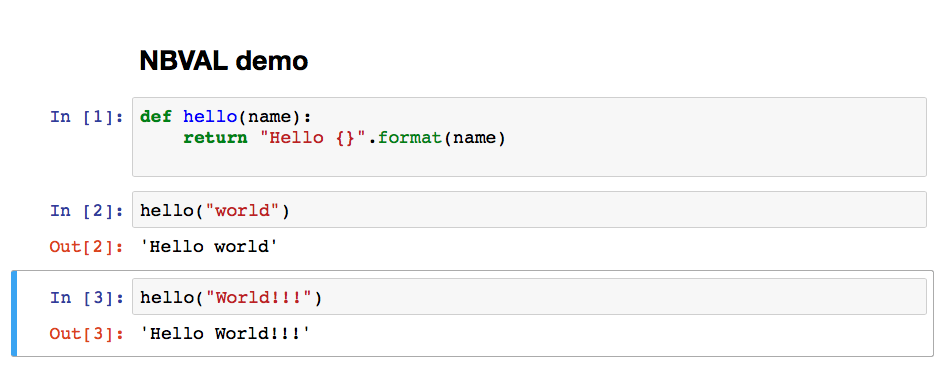
\includegraphics[width=1\textwidth]{examples/demo.png}
  \caption{Trivial notebook \texttt{demo.ipynb}. The code in cell [1] is
    representative of the computational package we use (typically
    accessed via the \texttt{import} statement).\label{fig:demo-ipynb}}
\end{figure}

Once the \nbval tool is installed (Section~\ref{sec:installation}), we
can use the\linebreak \texttt{py.test --nbval demo.ipynb} command to
validate the notebook with name
\texttt{demo.ipynb}. Figure~\ref{fig:demo-pytest} shows the output
from the testing process.

\begin{figure}[ht]
  \centering
  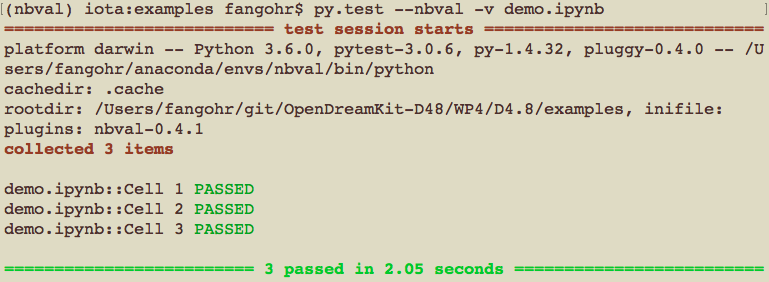
\includegraphics[width=1\textwidth]{examples/demo-pytest.png}
  \caption{\nbval Command and output from validating notebook
    \texttt{demo.ipynb} with \nbval. For each of the 3 cells in the notebook,
    the input code is re-executed, and any output compared with the
    output stored in the notebook file (see
    Figure~\ref{fig:demo-ipynb} for the notebook file).\label{fig:demo-pytest}}
\end{figure}


\subsection{Example 2}
We show another example where the code computes a different output
every time the notebook is run. This could be due to a change in the
software that is imported into the notebook, and might be something
that we want to report as an error. (There are other cases where we
like to ignore changing output - this is discussed in more detail in Section~\ref{sec:changing-outputs})

We use the notebook in figure~\ref{fig:demo-with-fail-ipynb} as an
example.

\begin{figure}[ht]
  \centering
  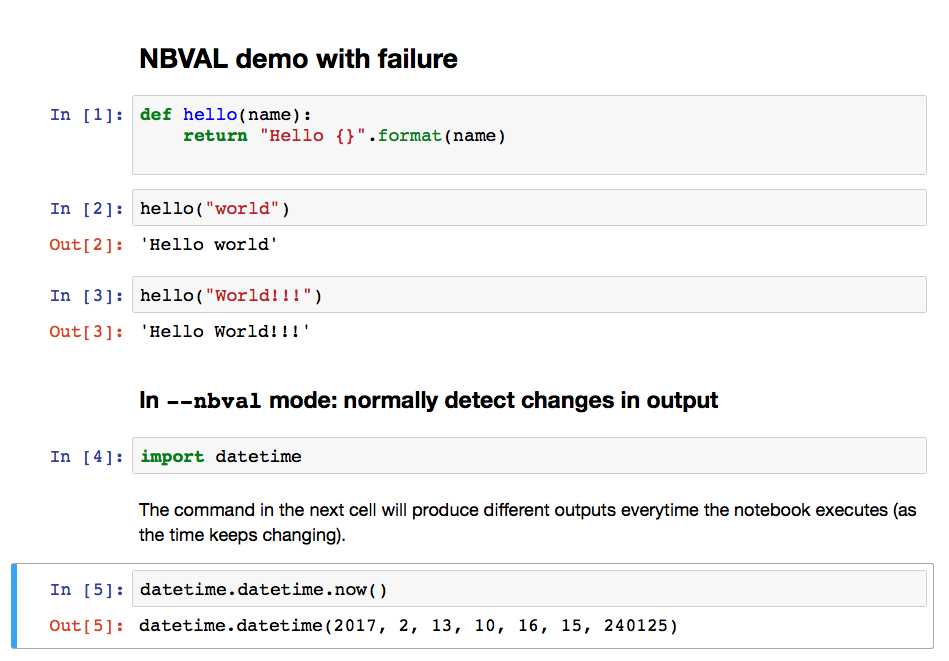
\includegraphics[width=1\textwidth]{examples/demo-with-fail.png}
  \caption{Trivial notebook \texttt{demo-with-fail.ipynb}. The code in
    cell [5] produces a different output every time the notebook
    executes as it reports the current date and time. \label{fig:demo-with-fail-ipynb}}
\end{figure}

As before, we trigger validation of the notebook with\linebreak \texttt{py.test --nbval demo-with-fail.ipynb}. Figure~\ref{fig:demo-with-fail-pytest} shows the output
from the testing process.

\begin{figure}[ht]
  \centering
  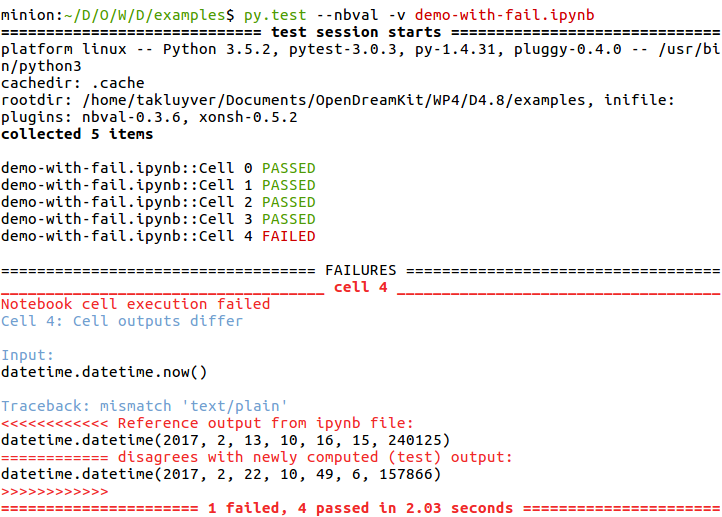
\includegraphics[width=1\textwidth]{examples/demo-with-fail-pytest.png}
  \caption{\nbval Command and output from validating notebook
    \texttt{demo-with-fail.ipynb} with \nbval. Cells [1], [2], [3],
    and [5] are code cells and produce output (although it could be
    \texttt{None}), and pass their tests. Cell [7] fails the test. The
    tool provides a detailed breakdown on what the output for cell [7]
    is in the stored file, and contrasts it with the output from the
    re-execution that has just taken place (see
    Figure~\ref{fig:demo-with-fail-ipynb} for the notebook
    file).\label{fig:demo-with-fail-pytest}}
\end{figure}

We can see that cells [1] to [5] pass tests, but cell [7] fails the test. The
tool provides a detailed breakdown on what the output for cell [7]
is in the stored file, and contrasts it with the output from the
re-execution that has just taken place.


% force floats to appear.
\clearpage
\subsection{Installation}\label{sec:installation}
The installation of the package is described as part of the
documenation available on Github
(https://github.com/computationalmodelling/nbval, in particular\linebreak
\href{https://github.com/computationalmodelling/nbval/blob/master/README.md}{https://github.com/computationalmodelling/nbval/blob/master/README.md}.)

Installation via \text{pip} in supported, which allows to install the
package in all Python installations.
\subsection{Documentation}
The detailed behaviour of the tool is described in the online
documentation\newline(\href{https://github.com/computationalmodelling/nbval/blob/master/documentation.ipynb}{https://github.com/computationalmodelling/nbval/blob/master/documentation.ipynb})
\subsection{Testing and continuous integration}
We have test suite with about 30 tests, that are executed
automatically using the Travis CI continuous integration service
(\href{https://travis-ci.org/computationalmodelling/nbval}{https://travis-ci.org/computationalmodelling/nbval}.)

We are testing for successful completion of the test suite for
Python versions 2.7, 3.5, 3.5, 3.6 and the nightly build of Python.

\section{Design}
\subsection{Overview}
\nbval (\url{https://github.com/computationalmodelling/nbval}) is a
new tool for testing notebooks, built as a plugin for the pytest
testing framework (\url{http://pytest.org}).  By leveraging existing
tools, \nbval fits well into the software development tools such as
continuous integration services and testing environments.

When \nbval encounters a notebook to test, it identifies the language
of the notebook from the notebook's metadata and starts a process to
run the code found in notebook, called the Kernel.  \nbval
communicates with this Kernel via the Jupyter protocol, as in the
notebook environment.  Each cell in a notebook constitutes a test, and
is executed in order, as if the notebook had been executed in the
interactive notebook environment.

Unlike traditional source code files, notebooks contain both code to
execute and the output.  Validating notebooks can take the output into
account or not.  At its most basic level, called `lax mode', \nbval
executes a cell, only checking for errors.  This verifies that
execution of a notebook completes without error, but makes no effort
to guarantee that the result is the same across executions.

\nbval's default mode is to record the output produced by executing
the notebook, and compare it with the output stored in the notebook.
At its strictest, any visible change in the output will result in a
failed test.  Many times, output can contain transient values that are
not informative, such as memory addresses or dates.  To deal with
this, \nbval provides an extensible mechanism for normalizing output,
so that these transient values may be excluded from the comparison
(see Section~\ref{sec:changing-outputs}).

\subsection{Implementation}

\nbval uses pytest, which is a popular, extensible testing framework for the Python language.
We use pytest because it is a standard tool for running tests in the Python community,
and enables extending functionality via a robust plugin system.
\nbval functions as a plugin for pytest, adding the following functionality:

\begin{itemize}
\item recognize Jupyter notebooks as files that could contain tests
\item construct and run tests based on notebook cells
\item report test results based on output, optionally with nbdime
\end{itemize}

One \nbval is installed, notebooks can be included in any pytest-based test suite
with a single \texttt{--nbval} argument.
Simiarly, collections of notebooks can be tested without any configuration by running
\texttt{pytest --nbval} in any directory containing notebooks.


\subsection{Changing outputs}\label{sec:changing-outputs}

One of the test features of \nbval that differs from traditional tests
is that notebooks contain the output produced by their previous execution.
One of the ways \nbval tests notebooks is by comparing outputs produced during the tests
with those recorded in the notebook.
Not all outputs are necessarily useful to test,
so \nbval provides some configuration for deciding which outputs should be tested,
and which should get some normalization before comparison.

The general mechanisms for less-than-exact output comparison are:

\begin{itemize}
\item mark cell to be ignored
\item use regular expressions
\item use nbval-lax
\end{itemize}

The output checking in \nbval may be controlled on a cell-by-cell
basis: notebook authors may either start with no output checking (`lax
mode') and mark specific cells whose output should be checked, or
start with full output checking and mark cells whose output should be
ignored.  The author indicate that nbval should not execute a cell at
all, or that it an error is the expected result of a cell.

\subsection{Exceptional behaviour}

There are three ways that a cell run as a test by nbval can result in a test
failure:

\begin{itemize}
\item The kernel reports that executing the cell contains an error,
and the cell is not marked as expected to produce an error.
\item The output from running a cell differs from that saved in a notebook,
nbval is not instructed to ignore that output,
and the changes are not covered by the regular expression patterns used to
normalise output.
\item Execution of the cell does not complete within a configurable timeout,
which by default is 2000 seconds.
\end{itemize}

In all three cases, the test corresponding to that cell is reported as a failure through pytest,
which will result in a description of the error being displayed to the user
(see Figure \ref{fig:nbval}).

\begin{figure}[ht]
  \centering
  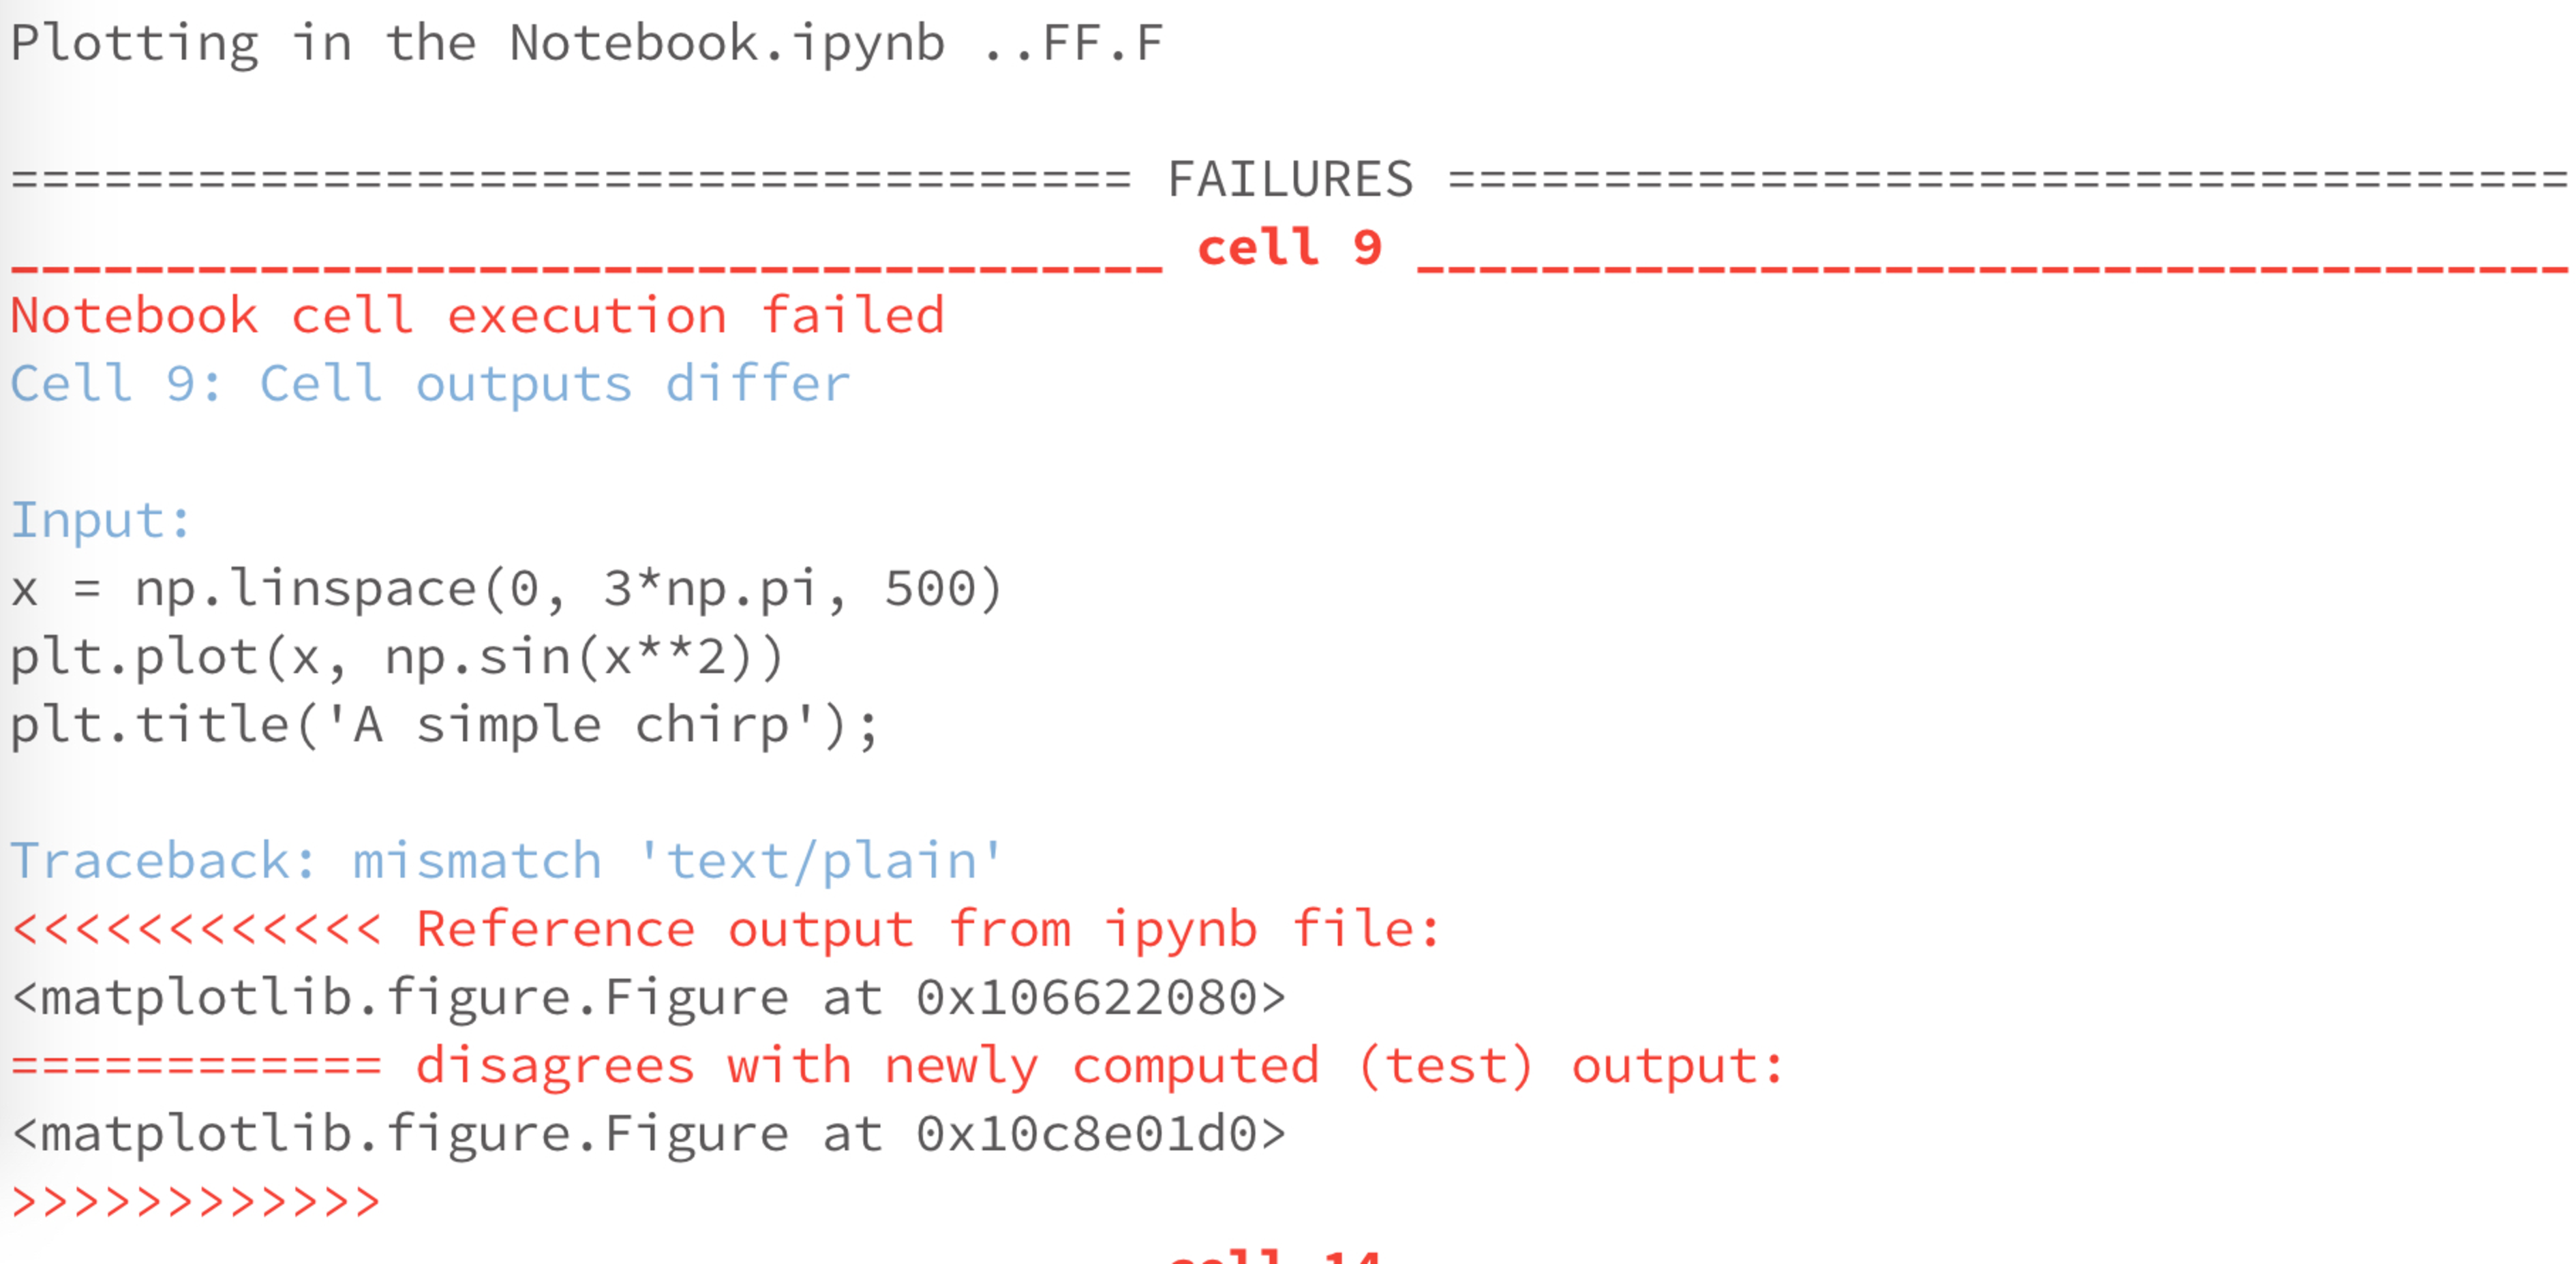
\includegraphics[width=1.0\textwidth]{img/nbval-terminal}
  \caption{\nbval output, showing that output changed.}\label{fig:nbval}
\end{figure}

When the failure is due to a difference in output,
\nbval can also optionally use nbdime to display how the notebook has changed
(see Section \ref{sec:nbval-nbdime}).

When the failure is due to a timeout executing code, execution is stopped.
Later cells in the same notebook are marked as `expected failures',
as later code often relies on the completion of earlier code,
and reporting several separate failures would obscure the underlying cause.


\subsection{Choice of kernel}

In the Jupyter protocol, a `kernel' is the process where code executes,
and is a separate process from the one reading the notebook and determining what code should be execute.
When kernels are installed on a system,
they register a `kernel spec' that describes how to start the kernel.
There can be many such kernels installed on a system,
some corresponding to different languages, such as GAP, PARI (\delivref{UI}{ipython-kernels}), Sage, or Python,
while others may correspond to particular environments.
Notebooks record information about the kernel used to run them in metadata.
\nbval can look at this metadata to select the appropriate kernel to run the notebook for tests.

When the notebook's code is Python,
Default kernel selection can be bypassed in \nbval to run the code with the same interpreter
with the \texttt{--current-env} flag.
This makes nbval fit best in testing frameworks,
which often create temporary environments in which to run tests.
The test code itself will execute in this environment,
but default kernel selection could result in the tests running in a different environment.
\texttt{--current-env} ensures that not only the test runner,
but the test code in the notebooks themselves,
is run in the test environment.


\subsection{Numbering of cells}

The Jupyter Notebook numbers code cells, in the order of
execution. These can be increasing integers starting from top of the
notebook to the bottom, for example if the cells are (written and)
executed in this order, or at a later point the user chooses to
restart the kernel, and run all cells in order. However, the notebook
also allows to execute cells in arbitrary order.

In contrast, With \nbval cells are always executed in order from start
to finish, and labelled with increasing integer numbers starting from
1.  This sequential execution enables \nbval to catch errors that may
not have been noticed due to out-of-order execution.

We note that \nbval counts all cells in the notebook, whereas the
notebook in the browser only counts code cells.
%TODO update if we change this behaviour


\section{\nbval and reproducibility} % (fold)

\nbval facilitates integrating notebooks into a reproducible
scientific workflow.  Tests are integral to maintaining and verifying
software, which is critical for validating and reproducing scientific
computation.  A publication can include a notebook that produces its
results or figures.  By using \nbval, the validation of this notebook
and output can be automated, to make it more convenient, and thus more
likely, for scientific publications to follow reproducible practices.


\section{\nbval and nbdime} % (fold)
\label{sec:nbval-nbdime}

\begin{figure}[ht]
  \centering
  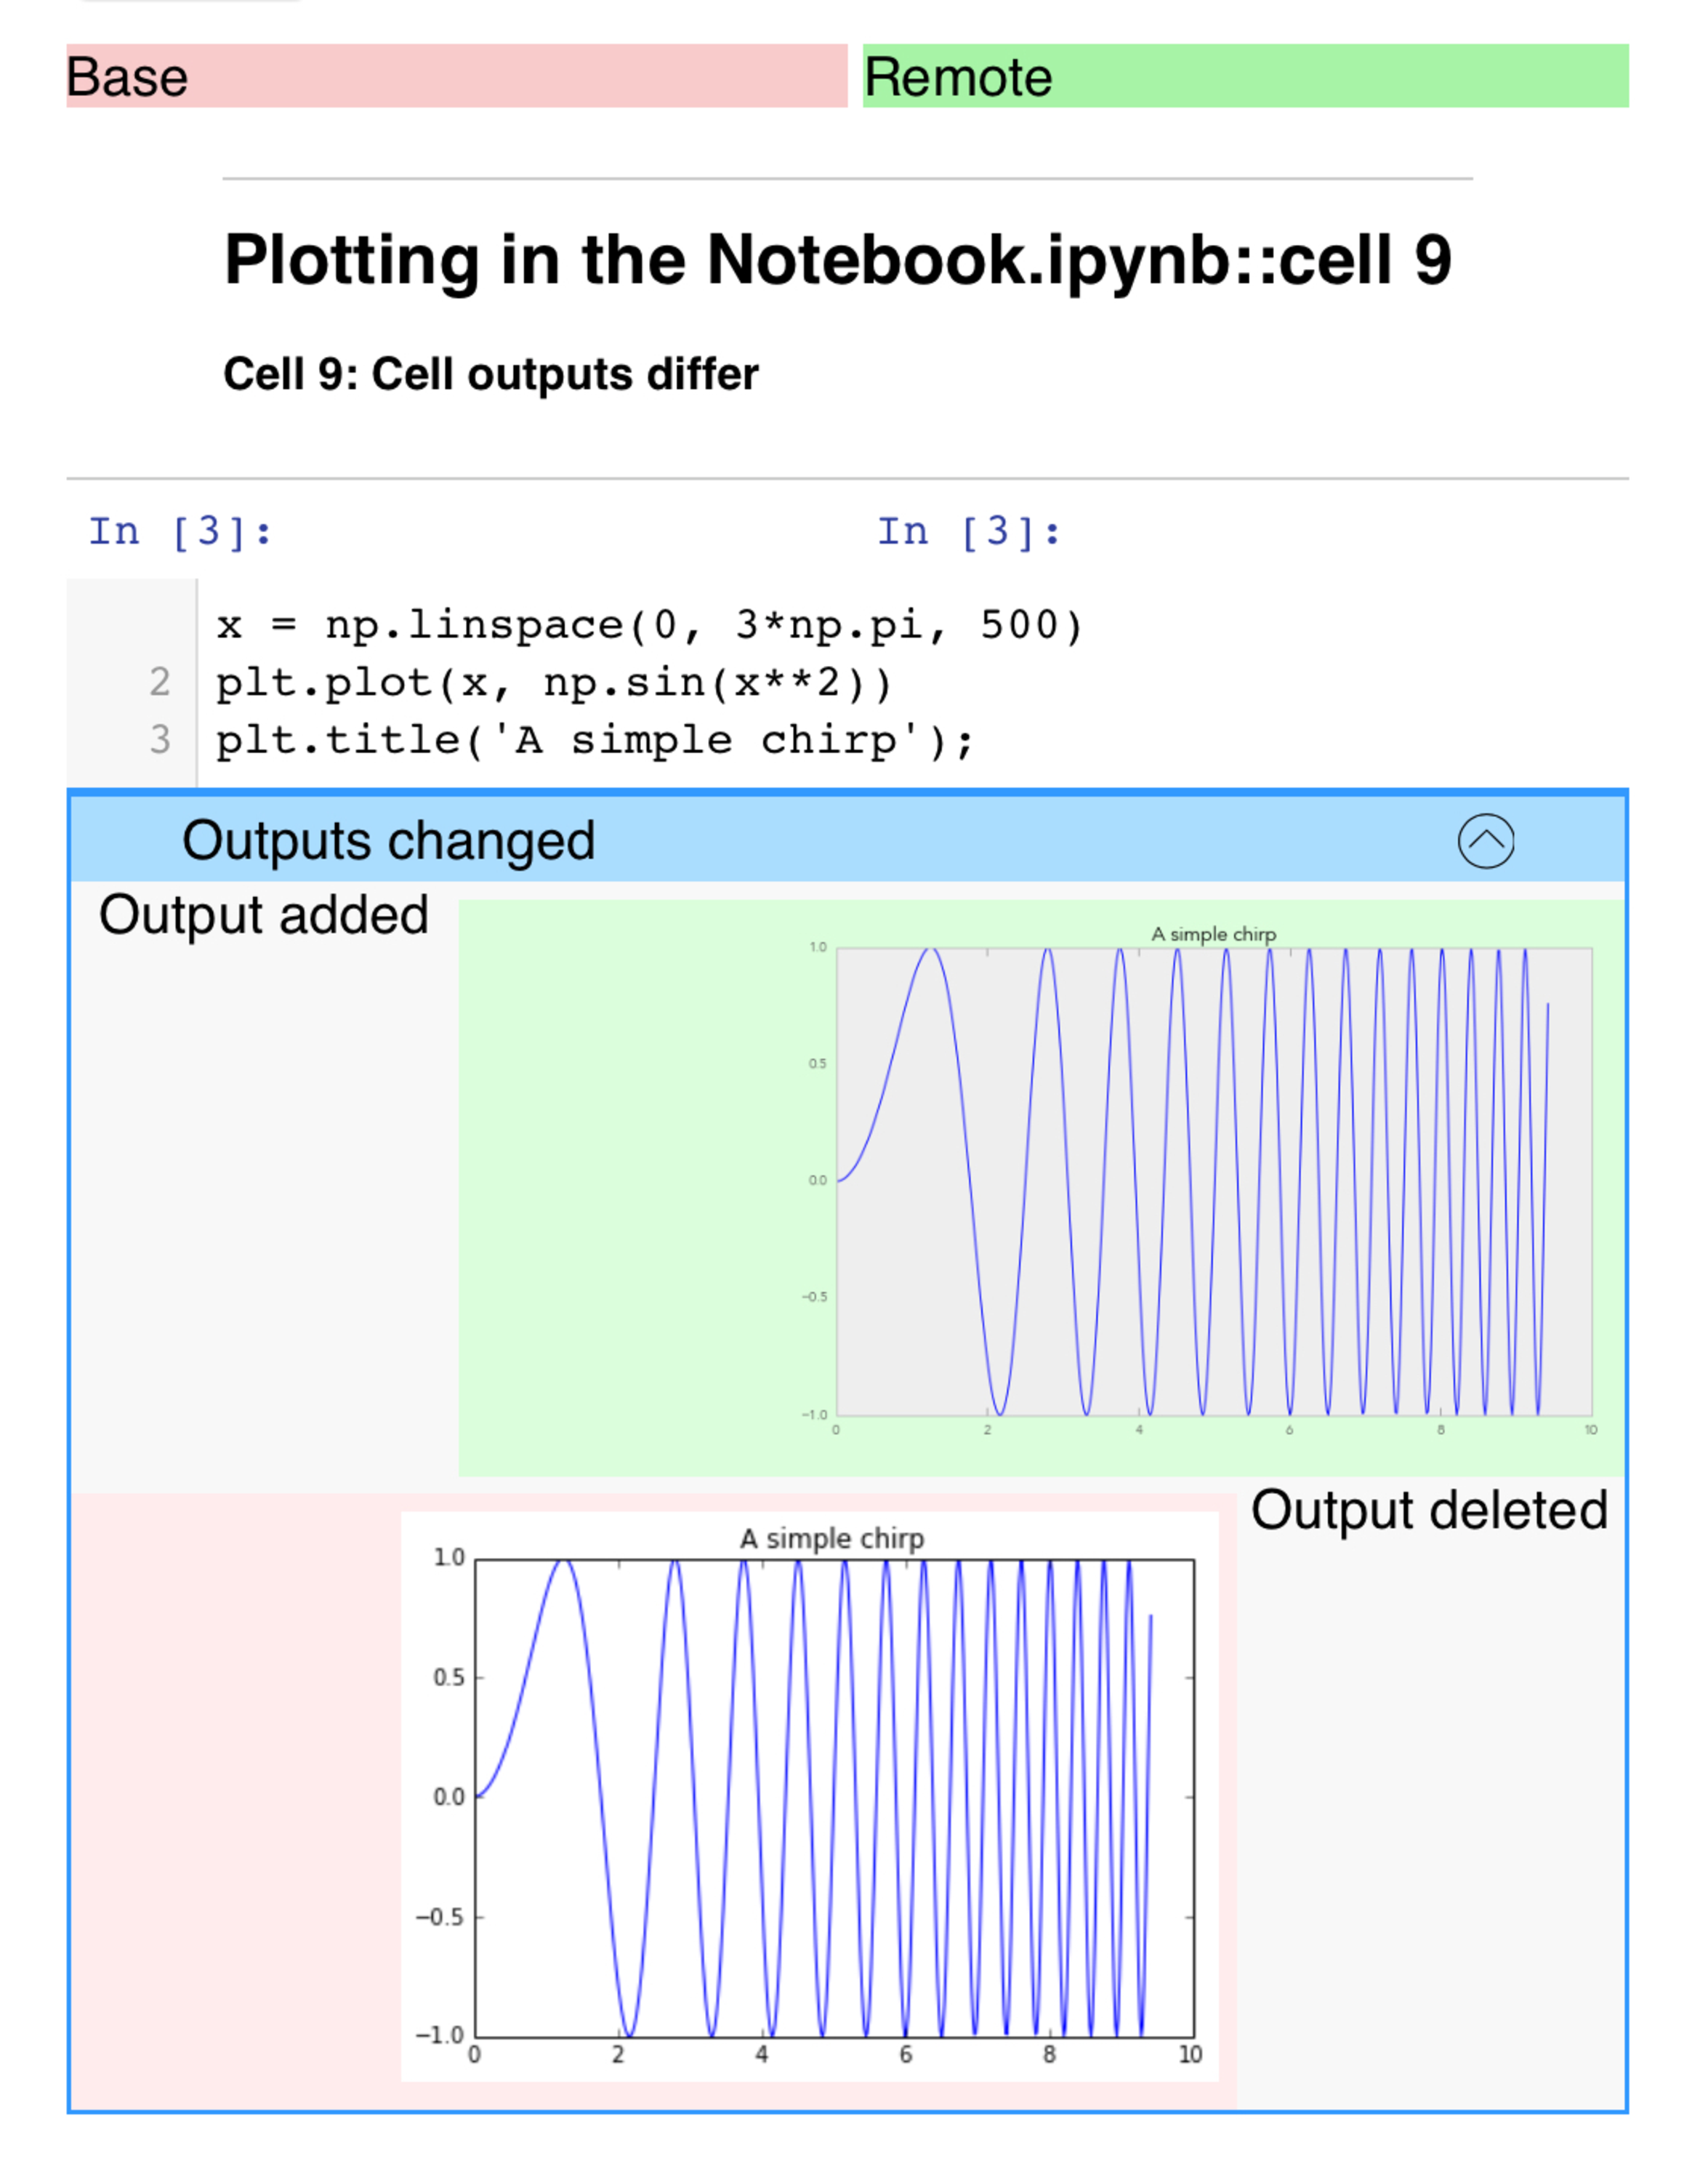
\includegraphics[width=.7\textwidth]{img/nbval-nbdime}
  \caption{An \nbval output rendered with \texttt{nbdime}}\label{fig:nbval-nbdime}
\end{figure}

Testing notebooks with \nbval involves comparing the notebook as saved,
and the notebook recently run.
This is comparing two notebooks,
which can build on earlier OpenDreamKit work.
\nbval can use nbdime, produced in \delivref{UI}{jupyter-collab},
to display the difference between the before and after notebooks,
for more effective comparison and identification of changes.

A graphical display allows humans to quickly take in a lot of
information, and intuitively spot visual differences between the
two documents, in particular when before and after images of
plots, graphs, and figures are shown.

\section{Usage reports}

As notebooks can be integrated directly into sphinx (and then be
hosted on \texttt{readthedocs}, for example), they are a convenient
way to create documentation for a software package.

Any examples that demonstrate interaction with the code are naturally
and efficiently included: the documentation developer just types the
command, the note book automatically displays the behaviour.

With \nbval, we can now include regression testing of the
documentation into the continuous integration, and will automatically
be alerted if the documented behaviour has changed (and thus the
documentation is outdated).

An example can be seen in this repository:
\href{https://github.com/joommf/oommfc}{https://github.com/joommf/oommfc},
which provides the documentation, for example at\linebreak
\href{http://oommfc.readthedocs.io/en/latest/ipynb/new_discretisedfield_interface.html}{http://oommfc.readthedocs.io/en/latest/ipynb/new\_discretisedfield\_interface.html}.

Being able to test the documentation \emph{automatically} addresses
the common scenario in which documentation is developed for the first
version of a tool, but not updated later, and increasingly getting out
of date. The package developers are unlikely to notice as they would
never read the documentation, in particular not the beginning aimed at
new users of the package. With \nbval one can integrate the regression
testing of the documentation into the continuous integration cycle.


\section{Future work} % (fold)

\nbval has been integrated successfully into some repositories of
notebook-based educational materials and software documentation by
OpenDreamKit participants, and is being integrated into the existing
notebook-based documentation of projects in the wider Jupyter
community.  We will work to encourage adoption of \nbval for verifying
documentation, and would like to see nbval used to enable verification
of scientific publications now that it has proved its effectiveness in
educational materials.

\printbibliography
\end{document}

%%% Local Variables:
%%% mode: latex
%%% TeX-master: t
%%% End:

%  LocalWords:  githubissuedescription newpage tableofcontents newpage printbibliography
